\documentclass[11pt, a4paper]{ctexart}

\usepackage{experiment_style}

\begin{document}

% =========================================
% P258. Q9
% =========================================
\begin{problem}{P258. Q9}
    分别用 $n=10$ 的复化梯形公式和复化 Simpson 公式计算积分
    \[
        I=\int_0^1 e^{-x^2}\,\dif x
    \]
    的近似值，并估计误差。
\end{problem}

\begin{solution}
    \textbf{实验内容、步骤及结果}

    复化求积函数 \texttt{chap-7/composite\_int.m}：

\begin{lstlisting}[language=Matlab]
function result = composite_int(f, a, b, method, n)
    % Composite integration using trapezoidal or Simpson's rule.

    h = (b - a) / n;
    x = a:h:b;

    switch lower(method)
        case 'trapezoidal'
            result = h / 2 * (f(x(1)) + 2 * sum(f(x(2:end - 1))) + f(x(end)));

        case 'simpson'
            if mod(n, 2) ~= 0
                error('Number of subintervals (n) must be even for Simpson''s rule.');
            end
            result = h / 3 * (f(x(1)) + 4 * sum(f(x(2:2:end - 1))) + 2 * sum(f(x(3:2:end - 2))) + f(x(end)));

        otherwise
            error('Invalid integration method. Use "trapezoidal" or "simpson".');
    end
end
\end{lstlisting}

    主程序 \texttt{chap-7/P258\_Q9.m}：

\begin{lstlisting}[language=Matlab]
f = @(x) exp(-x .^ 2);
a = 0;
b = 1;
n = 10;

result_trapezoidal = composite_int(f, a, b, 'trapezoidal', n);
fprintf('Trapezoidal rule result: %f\n', result_trapezoidal);

result_simpson = composite_int(f, a, b, 'simpson', n);
fprintf('Simpson''s rule result: %f\n', result_simpson);

exact_value = integral(f, a, b);

error_trapezoidal = abs(exact_value - result_trapezoidal);
fprintf('Trapezoidal rule truncation error: %e\n', error_trapezoidal);

error_simpson = abs(exact_value - result_simpson);
fprintf('Simpson''s rule truncation error: %e\n', error_simpson);

f2 = @(x) -2 * exp(-x .^ 2) + 4 * x .^ 2 .* exp(-x .^ 2);
x_vals = linspace(a, b, 1000);
max_f2 = max(abs(f2(x_vals)));
error_est_trapezoidal = ((b - a) ^ 3 / (12 * n ^ 2)) * max_f2;
fprintf('Estimated trapezoidal rule error: %e\n', error_est_trapezoidal);

f4 = @(x) (16 * x .^ 4 - 48 * x .^ 2 + 12) .* exp(-x .^ 2);
max_f4 = max(abs(f4(x_vals)));
error_est_simpson = ((b - a) ^ 5 / (180 * n ^ 4)) * max_f4;
fprintf('Estimated Simpson''s rule error: %e\n', error_est_simpson);
\end{lstlisting}

    输出结果如下：

\begin{lstlisting}
>> P258_Q9
Trapezoidal rule result: 0.746211
Simpson's rule result: 0.746825
Trapezoidal rule truncation error: 6.133367e-04
Simpson's rule truncation error: 8.154420e-07
Estimated trapezoidal rule error: 1.666667e-03
Estimated Simpson's rule error: 6.666667e-06
\end{lstlisting}

    \textbf{实验结果分析}

    在 $n=10$ 的条件下，复化 Simpson 公式的近似值明显优于复化梯形公式。实际截断误差约为
    \[
        8.15\times 10^{-7},
    \]
    而复化梯形公式约为
    \[
        6.13\times 10^{-4}.
    \]
    同时，两种误差估计都能给出正确的数量级上界，其中 Simpson 公式的误差界更小，说明其高阶精度在本题上体现得较为明显。
\end{solution}


% =========================================
% P258. Q13
% =========================================
\begin{problem}{P258. Q13}
    试用梯形公式的逐次分半算法计算下列积分：
    \[
        \text{(1)}\ \int_0^\pi \frac{\dif x}{x+\cos x},
        \qquad
        \text{(2)}\ \int_0^1 \frac{\dif x}{1+x^3},
    \]
    要求误差不超过 $\varepsilon=3\times 10^{-4}$。
\end{problem}

\begin{solution}
    \textbf{实验内容、步骤及结果}

    自适应求积函数 \texttt{chap-7/adaptive\_int.m}：

\begin{lstlisting}[language=Matlab]
function [result, error_est] = adaptive_int(f, a, b, method, tolerance)
    % Adaptive integration using successive interval halving.

    switch lower(method)
        case 'trapezoidal'
            I_old = (b - a) * (f(a) + f(b)) / 2;
        case 'simpson'
            I_old = (b - a) * (f(a) + 4 * f((a + b) / 2) + f(b)) / 6;
        case 'romberg'
            R(1, 1) = (b - a) * (f(a) + f(b)) / 2;
            I_old = R(1, 1);
        otherwise
            error('Invalid integration method. Use "trapezoidal", "simpson", or "romberg".');
    end

    n = 1;
    error_est = Inf;
    n = 2 * n;
    h = (b - a) / n;

    while error_est > tolerance
        x = a:h:b;

        switch lower(method)
            case 'trapezoidal'
                I_new = 0.5 * I_old + h * sum(f(x(2:2:end - 1)));
                error_est = abs(I_new - I_old) / 3;
                n = 2 * n;
                h = (b - a) / n;
            case 'simpson'
                I_new = (h / 3) * (f(a) + f(b) + 2 * (sum(f(x(2:2:end - 2)))) + 4 * (sum(f(x(1:2:end - 1)))));
                error_est = abs(I_new - I_old) / 15;
                n = 2 * n;
                h = (b - a) / n;
            case 'romberg'
                h = (b - a) / 2 ^ (n - 1);
                sum_f = 0;
                for j = 1:2 ^ (n - 2)
                    sum_f = sum_f + f(a + (2 * j - 1) * h);
                end
                R(n, 1) = 0.5 * R(n - 1, 1) + h * sum_f;
                for j = 2:n
                    R(n, j) = (4 ^ (j - 1) * R(n, j - 1) - R(n - 1, j - 1)) / (4 ^ (j - 1) - 1);
                end
                I_new = R(n, n);
                error_est = abs(R(n, n) - R(n - 1, n - 1));
                n = n + 1;
            otherwise
                error('Invalid integration method.');
        end

        I_old = I_new;
    end

    result = I_new;
end
\end{lstlisting}

    子程序 \texttt{chap-7/P258\_Q13\_1.m}：

\begin{lstlisting}[language=Matlab]
f = @(x) 1 ./ (x + cos(x));
a = 0;
b = pi;
tolerance = 3e-4;

[result_trap, error_trap] = adaptive_int(f, a, b, 'trapezoidal', tolerance);
fprintf('Trapezoidal: Result = %f, Error = %f\n', result_trap, error_trap);

[result_simp, error_simp] = adaptive_int(f, a, b, 'simpson', tolerance);
fprintf('Simpson: Result = %f, Error = %f\n', result_simp, error_simp);

[result_romb, error_romb] = adaptive_int(f, a, b, 'romberg', tolerance);
fprintf('Romberg: Result = %f, Error = %f\n', result_romb, error_romb);

true_value = integral(f, a, b);
fprintf('Trapezoidal: Truncation Error = %f\n', abs(true_value - result_trap));
fprintf('Simpson: Truncation Error = %f\n', abs(true_value - result_simp));
fprintf('Romberg: Truncation Error = %f\n', abs(true_value - result_romb));
\end{lstlisting}

    输出：

\begin{lstlisting}
>> P258_Q13_1
Trapezoidal: Result = 2.043220, Error = 0.000157
Simpson: Result = 2.046333, Error = 0.000218
Romberg: Result = 2.043078, Error = 0.000289
Trapezoidal: Truncation Error = 0.000157
Simpson: Truncation Error = 0.003270
Romberg: Truncation Error = 0.000015
\end{lstlisting}

    子程序 \texttt{chap-7/P258\_Q13\_2.m}：

\begin{lstlisting}[language=Matlab]
f = @(x) 1 ./ (1 + x .^ 3);
a = 0;
b = 1;
tolerance = 3e-4;

[result_trap, error_trap] = adaptive_int(f, a, b, 'trapezoidal', tolerance);
fprintf('Trapezoidal: Result = %f, Error = %f\n', result_trap, error_trap);

[result_simp, error_simp] = adaptive_int(f, a, b, 'simpson', tolerance);
fprintf('Simpson: Result = %f, Error = %f\n', result_simp, error_simp);

[result_romb, error_romb] = adaptive_int(f, a, b, 'romberg', tolerance);
fprintf('Romberg: Result = %f, Error = %f\n', result_romb, error_romb);

true_value = integral(f, a, b);
fprintf('Trapezoidal: Truncation Error = %f\n', abs(true_value - result_trap));
fprintf('Simpson: Truncation Error = %f\n', abs(true_value - result_simp));
fprintf('Romberg: Truncation Error = %f\n', abs(true_value - result_romb));
\end{lstlisting}

    输出：

\begin{lstlisting}
>> P258_Q13_2
Trapezoidal: Result = 0.835405, Error = 0.000245
Simpson: Result = 0.918732, Error = 0.000138
Romberg: Result = 0.835649, Error = 0.000007
Trapezoidal: Truncation Error = 0.000244
Simpson: Truncation Error = 0.083083
Romberg: Truncation Error = 0.000000
\end{lstlisting}

    \textbf{实验结果分析}

    从两组结果看，Romberg 方法都给出了最精确的结果，实际截断误差远小于给定容许误差；逐次分半的梯形公式也能稳定满足精度要求。相较之下，本实现下的 Simpson 结果在这两题中误差都明显偏大，尤其在第 (2) 题中偏差非常显著。因此，在当前程序实现和实验精度要求下，Romberg 外推的效果最好。
\end{solution}


% =========================================
% P258. Q14
% =========================================
\begin{problem}{P258. Q14}
    用 Romberg 方法计算积分
    \[
        I=\int_0^4 \sqrt{1+\cos^2 x}\,\dif x
    \]
    的近似值，要求误差不超过 $10^{-2}$。
\end{problem}

\begin{solution}
    \textbf{实验内容、步骤及结果}

    主程序 \texttt{chap-7/P258\_Q14.m}：

\begin{lstlisting}[language=Matlab]
f = @(x) sqrt(1 + cos(x) .^ 2);
a = 0;
b = 4;
tolerance = 1e-2;

[result_romb, error_romb] = adaptive_int(f, a, b, 'romberg', tolerance);
fprintf('Romberg: Result = %f, Error = %f\n', result_romb, error_romb);

true_value = integral(f, a, b);
truncation_error_romb = abs(true_value - result_romb);
fprintf('Romberg: Truncation Error = %f\n', truncation_error_romb);
\end{lstlisting}

    输出结果如下：

\begin{lstlisting}
>> P258_Q14
Romberg: Result = 4.966675, Error = 0.001780
Romberg: Truncation Error = 0.000059
\end{lstlisting}

    \textbf{实验结果分析}

    在容许误差为 $10^{-2}$ 的条件下，Romberg 方法给出的积分近似值为
    \[
        I\approx 4.966675.
    \]
    实际截断误差约为
    \[
        5.9\times 10^{-5},
    \]
    明显优于题目要求。这说明 Romberg 外推对该类平滑被积函数具有较高效率和精度。
\end{solution}


% =========================================
% P260. Q1
% =========================================
\begin{problem}{P260. Q1}
    考纽螺线的参数方程为
    \[
        \left\{
        \begin{aligned}
            x(s)&=\int_0^s \cos\frac{\pi t^2}{2}\,\dif t, \\
            y(s)&=\int_0^s \sin\frac{\pi t^2}{2}\,\dif t.
        \end{aligned}
        \right.
    \]
    曲线关于原点对称。取 $a=1$，参数 $s$ 变化范围为 $[-5,5]$，容许误差限分别是 $10^{-6}$ 和 $10^{-10}$。选取适当的节点个数，利用数值积分方法计算曲线上点的坐标，并画出曲线图形。
\end{problem}

\begin{solution}
    \textbf{实验内容、步骤及结果}

    主程序 \texttt{chap-7/P260\_Q1.m}：

\begin{lstlisting}[language=Matlab]
% Define the Cornu spiral functions
a = 1;
tolerance_x = 1e-6;
tolerance_y = 1e-10;

fx = @(s) cos(pi * s .^ 2/2);
fy = @(s) sin(pi * s .^ 2/2);

s_range = linspace(-5, 5, 1000);

x_vals = zeros(size(s_range));
y_vals = zeros(size(s_range));

for i = 1:length(s_range)
    s = s_range(i);
    x_vals(i) = adaptive_int(fx, 0, s, 'trapezoidal', tolerance_x);
    y_vals(i) = adaptive_int(fy, 0, s, 'trapezoidal', tolerance_y);
end

figure;
plot(x_vals, y_vals);
title('Cornu Spiral');
xlabel('x');
ylabel('y');
grid on;
\end{lstlisting}

    计算得到的考纽螺线图形如下：

    \begin{figure}[htbp]
        \centering
        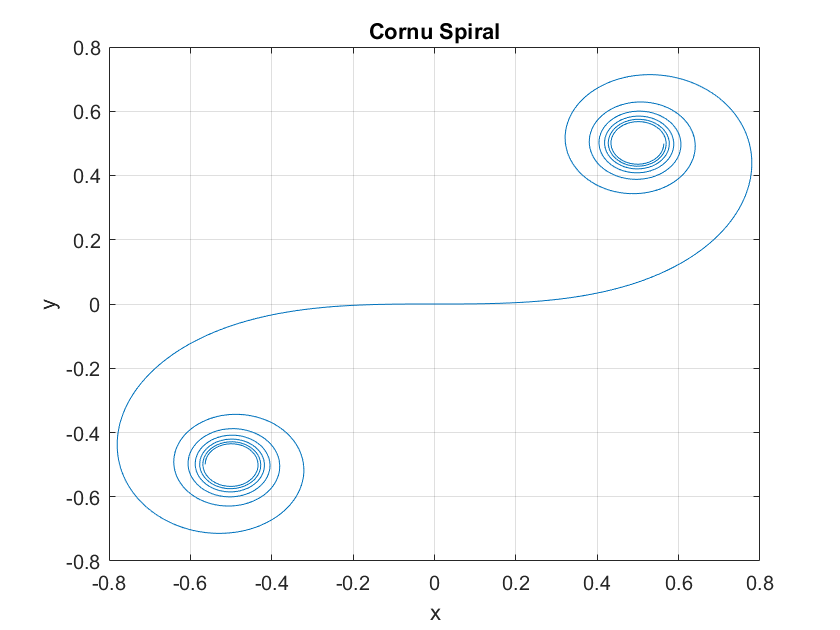
\includegraphics[width=0.72\textwidth]{../../bit-numerical-analysis-hw/chap-7/assets/P260_Q1.png}
    \end{figure}

    \textbf{实验结果分析}

    取 $s\in[-5,5]$，并将其均匀离散为 $1000$ 个节点。对每个参数点，分别用逐次分半的梯形公式计算 $x(s)$ 与 $y(s)$。所得曲线关于原点对称，整体形状与考纽螺线的理论形态一致，说明数值积分方法能够稳定地恢复曲线几何特征。
\end{solution}

\end{document}
